\documentclass[hyperref={colorlinks = true,linkcolor = blue, citecolor=blue,urlcolor=blue}]{beamer}  
\usetheme{default}

\usepackage{amsthm,amsmath,amssymb}
\usepackage{dsfont}
\usepackage{graphicx}
\usepackage{natbib}
\usepackage[space]{grffile}
\usepackage{booktabs}


\title{The Impact of Natural Disasters on Education: \\ Evidence from Standardized Testing}
\author{Gregor Steiner}
\date{July 11, 2022}

\begin{document}
		
\begin{frame}[plain]
    \maketitle
\end{frame}

\begin{frame}{Introduction}
	I exploit quasi-random variation in natural disaster exposure in the United States to answer two questions:
	\begin{itemize}
		\item \textbf{What is the causal effect of natural disasters on academic achievement as measured by standardized test scores?}
		\item What is the role of federal disaster assistance? Which counties apply for assistance?
	\end{itemize}
	\textbf{Why is this important?}\\
	Negative effects in education affect earnings
	potential $\implies$ Inequality in disaster risk exposure could exacerbate economic inequality
\end{frame}

\begin{frame}{Data}
	\begin{itemize}
		\item \textbf{Natural disasters}:
		\begin{itemize}
			\item Federal Emergency Management Agency (FEMA) declarations 
			\item Storms from the National Weather Service (NWS)
			\item Daily temperature data from the Global Historical Climatology Network
		\end{itemize}
		\item \textbf{Standardized testing outcomes} from the Stanford Education Data Archive \citep{SEDA}:
		\begin{itemize}
			\item Cohort standardized average scores by county in Mathematics \& Reading Language Arts (RLA)
			\item Grades 3 through 8 for schoolyears 2008-09 to 2017-18
		\end{itemize}
		\item \textbf{Public Assistance applications and payments} from FEMA
	\end{itemize}
\end{frame}

\begin{frame}{Distribution of mean test scores by subgroup}
	\begin{figure}[!h]
		\centering
		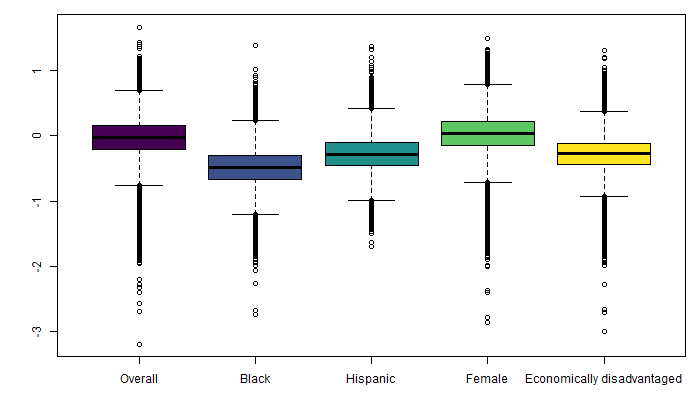
\includegraphics[scale=0.68]{"../Code & Data/DepVarsBoxplot.pdf"}
		\caption{Boxplots of mean test scores by subgroup}
		\label{DepVarsBoxplot}
	\end{figure}
\end{frame}


\begin{frame}{Natural Disasters in the US}
	\begin{figure}[!h]
		\centering
		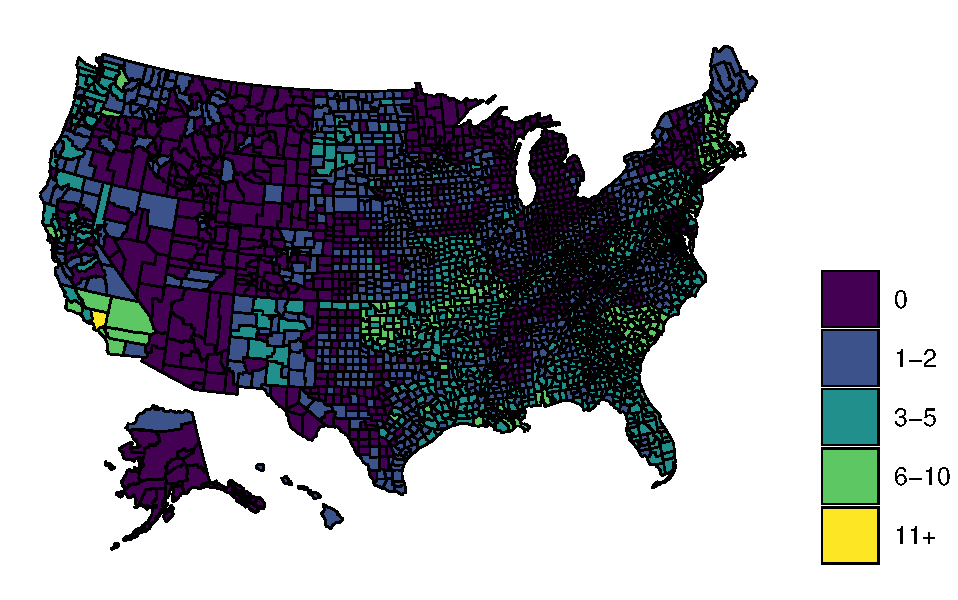
\includegraphics[scale=0.65]{"../Code & Data/DisasterMap.pdf"}
		\caption{Number of declared natural disasters in school years 2008-09 through 2017-18}
		\label{DisasterMap}
	\end{figure}
\end{frame}

\begin{frame}{When do counties apply for assistance?}
	\small
	\begin{table}

\caption{\label{tab:AppsByType}Share of counties that applied for federal assistance following a disaster by disaster type (schoolyears 2016-17 and 2017-18)}
\centering
\begin{tabular}[t]{lrr}
\toprule
  & Number of Cases & Applied for Assistance (in \%)\\
\midrule
Coastal Storm & 3 & 33.33\\
Dam/Levee Break & 3 & 0.00\\
Fire & 100 & 11.00\\
Flood & 270 & 41.85\\
Hurricane & 1217 & 23.25\\
Mud/Landslide & 22 & 50.00\\
Severe Ice Storm & 20 & 0.00\\
Severe Storm(s) & 164 & 28.66\\
Snow & 36 & 8.33\\
Tornado & 29 & 79.31\\
\addlinespace
Total & 1864 & 26.39\\
\bottomrule
\end{tabular}
\end{table}

\end{frame}

\begin{frame}{Which counties apply for assistance?}
	\begin{figure}[!h]
		\centering
		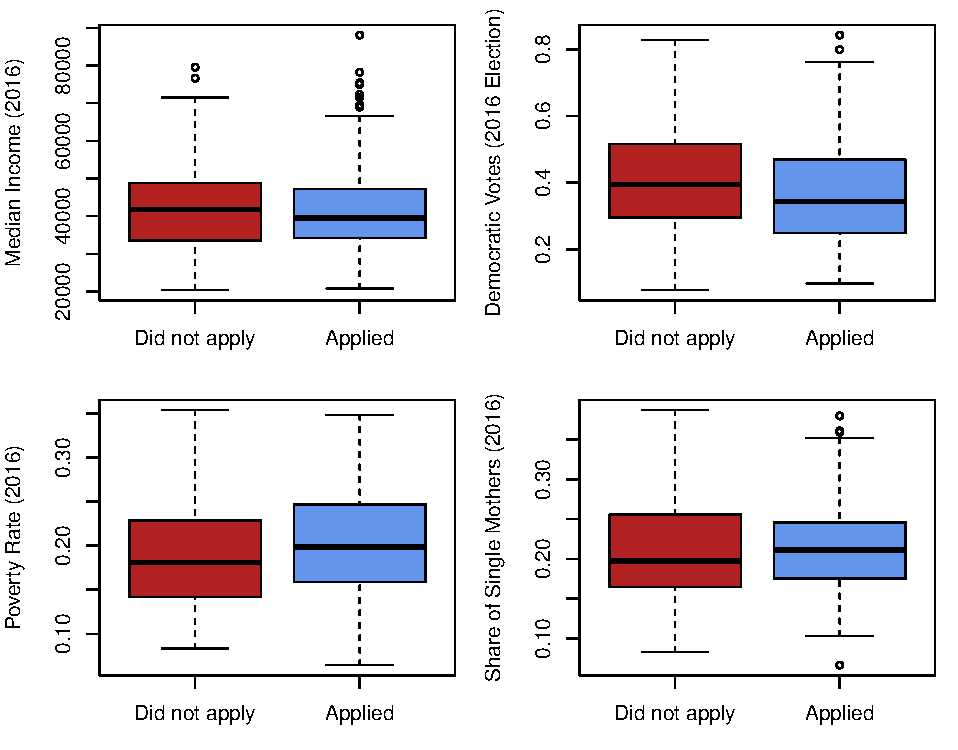
\includegraphics[scale=0.58]{"../Code & Data/AssistanceCovBoxplot.pdf"}
		\caption{Boxplots by application status}
		\label{AssistCovBoxplot}
	\end{figure}
\end{frame}

\begin{frame}{Empirical Strategy}
	\begin{itemize}
		\item Event-study design:
		\begin{align*}
			y_{i, t, g} &= \beta_{-5}  \mathds{1}\{t - E_i \leq 5\} + \sum_{l = -4, \; l \neq -1}^{8} \beta_l \mathds{1}\{t - E_i = l\} \\ &+ \alpha_i + \lambda_t + \zeta_g + \varepsilon_{i, t, g}
		\end{align*}
		\item Treatment begins in the period of first disaster ($E_i$) and is absorbing (staggered adoption)
		\item But: Always-treated (i.e. disaster in the first year) counties are dropped
		\item Never-treated counties act as the baseline
		\item Standard-errors clustered at the cohort level \citep{Abadie_2017}
	\end{itemize}
\end{frame}

\begin{frame}{Empirical Strategy: Identification}
	\begin{itemize}
		\item Natural disasters are plausibly independent of unobserved determinants of test scores conditional on location and year
		\item Heterogenous treatment effects $\implies$ simple TWFE is inadequate \citep{deChaisemartin_2020, Sun_2021}
		\item Solution: Interaction-Weighted Estimator (IW) by \cite{Sun_2021}
		\item Identifying Assumptions: Parallel Trends \& No Anticipatory Behavior
		\item IW consistently estimates a weighted average of cohort average treatment effects on the treated (CATT)
	\end{itemize}
\end{frame}

\begin{frame}{Main Results: FEMA}
	\begin{figure}[!h]
		\centering
		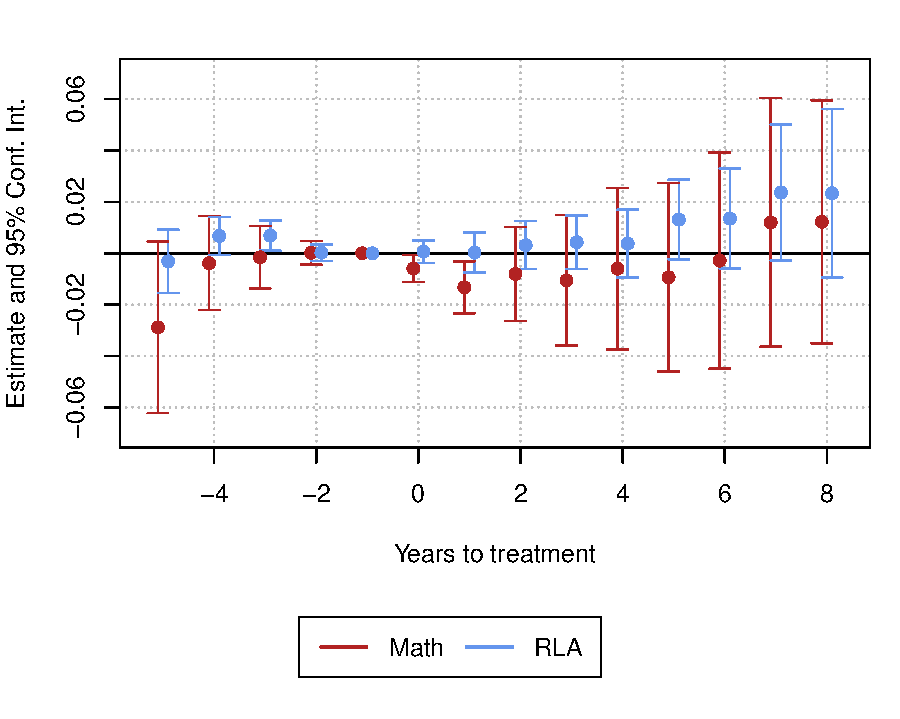
\includegraphics[scale=0.6]{"../Code & Data/ResultsPlotPresentation.pdf"}
		\caption{Dynamic Treatment effects in relative time: FEMA disaster data}
	\end{figure}
\end{frame}


\begin{frame}{Main Results: Subgroups, FEMA}
	\begin{figure}[!h]
		\centering
		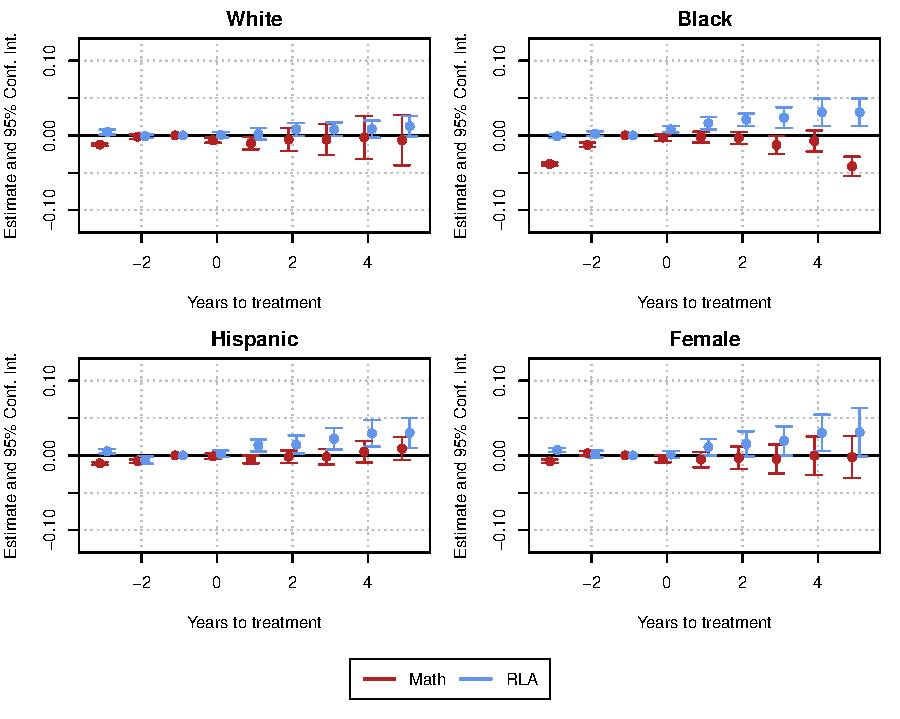
\includegraphics[scale=0.6]{"../Code & Data/ResultsPlotPresentationSubgroups.pdf"}
		\caption{Dynamic Treatment effects in relative time: FEMA disaster data}
	\end{figure}
\end{frame}


\begin{frame}{Main Results: Storms}
	\begin{figure}[!h]
		\centering
		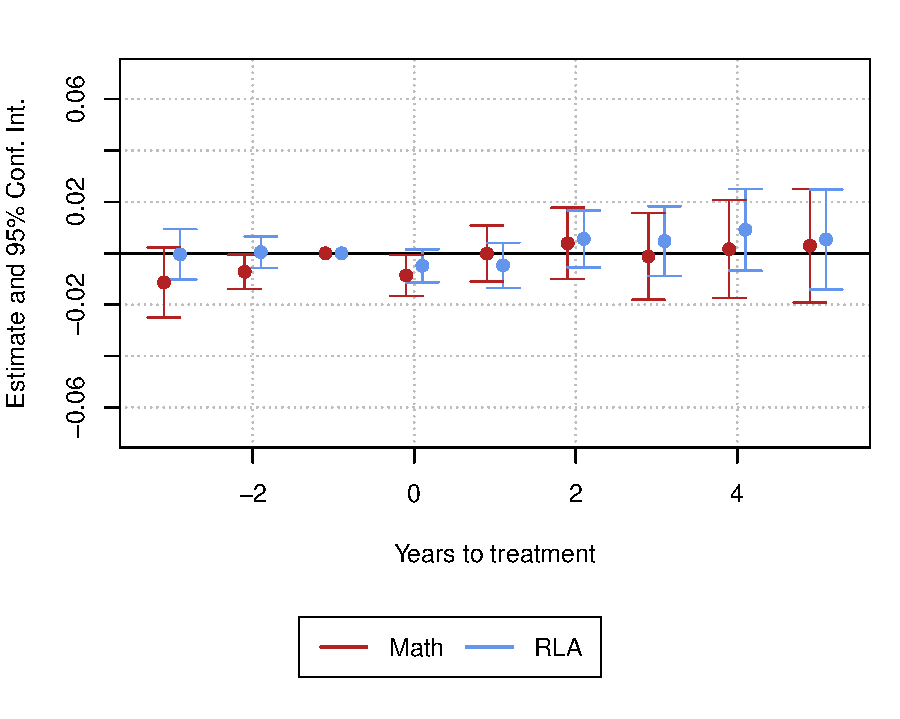
\includegraphics[scale=0.6]{"../Code & Data/ResultsPlotStormsPresentation.pdf"}
		\caption{Dynamic Treatment effects in relative time: NWS storm data}
	\end{figure}
\end{frame}


\begin{frame}{Main Results: Subgroups, Storms}
	\begin{figure}[!h]
		\centering
		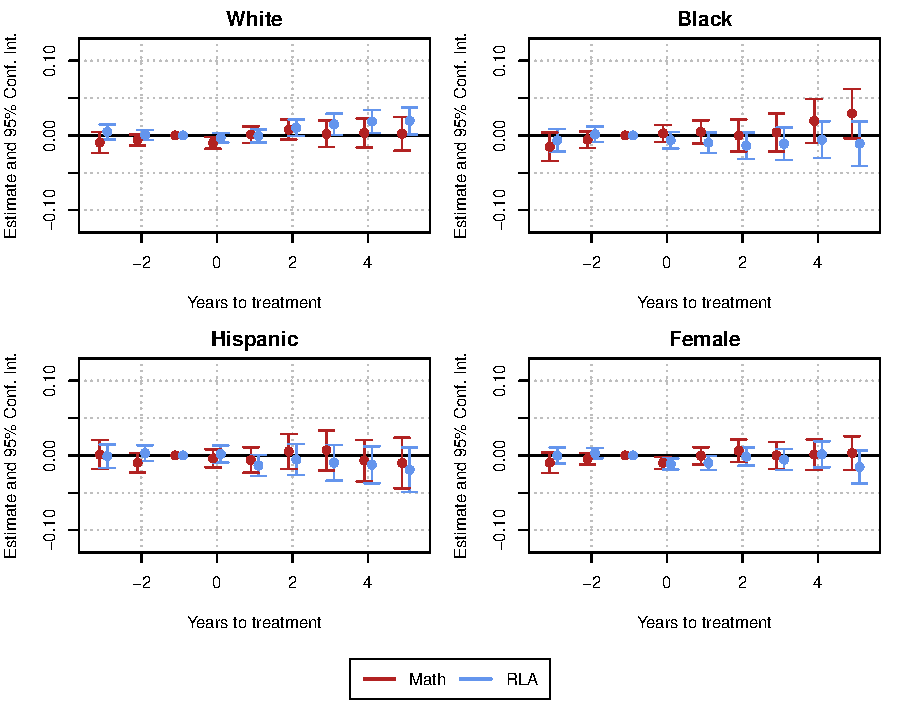
\includegraphics[scale=0.6]{"../Code & Data/ResultsPlotStormsPresentationSubgroups.pdf"}
		\caption{Dynamic Treatment effects in relative time: NWS storm data}
	\end{figure}
\end{frame}


\begin{frame}{Are these results driven by changes in county composition?}
	
	\begin{figure}[!h]
		\centering
		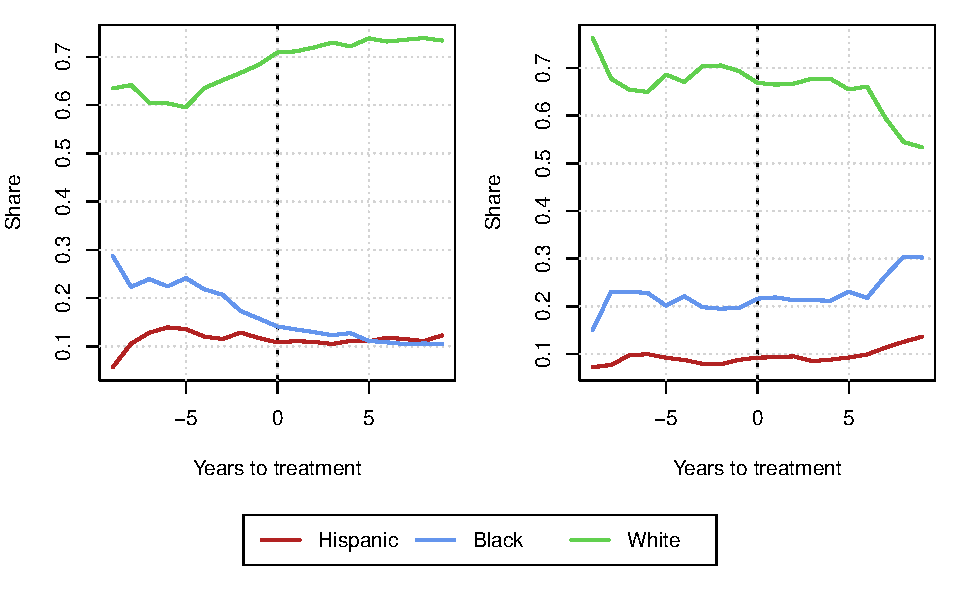
\includegraphics[scale=0.6]{"../Code & Data/EthnicComposition.pdf"}
		\caption{Aggregated ethnic shares by treatment timing based on FEMA disasters (left) and on NWS storms (right)}
		\label{EthnicComposition}
	\end{figure}
\end{frame}


\begin{frame}{Conclusion}
	\begin{itemize}
		\item Negative short-term effect of disasters on achievement in mathematics
		\item Some positive long-term effects among subgroups (but not very robust)
		\item Socially vulnerable counties are more likely to need federal assistance following a disaster
	\end{itemize}
\end{frame}



\begin{frame}{References}
	% bibliography
	\bibliographystyle{apalike}
	\bibliography{references}
\end{frame}




\end{document}
